%%%% PLEASE REPLACE ENTIRELY WITH YOUR OWN CONTENT %%%%


\chapter{Metodologia / desenvolupament del projecte}
  
  En aquest capítol es detallarà la metodologia emprada en la realització del treball. Té com a objectiu oferir un compte detallat de les aproximacions i tècniques utilitzades, assegurant la replicabilitat i el rigor acadèmic. No només cobrirà els mètodes de recerca i tècniques de mesurament emprats, sinó que també aprofundirà en les especificitats del desenvolupament de programari i maquinari. Tant si el projecte implica anàlisi qualitativa, mesuraments quantitatius, modelatge computacional com prototipatge físic, aquest capítol hauria d'elucidar com contribueix cada component als objectius generals.
  
  A més de descriure els mètodes en si mateixos, el capítol també proporcionarà justificacions per què es van escollir mètodes particulars enfront d'altres. Per exemple, podria explicar la tria d'un llenguatge de programació específic, prova estadística o configuració experimental. El capítol també abordarà les limitacions de la metodologia i com aquestes s'han mitigat o tingut en compte. Els lectors haurien de sortir amb una comprensió clara de com s'ha dut a terme el desenvolupament del projecte, per què s'han escollit determinades opcions i com aquests mètodes serveixen per complir els objectius establerts inicialment.

\section{Escenari utilitzat}

  L’escenari presentat en aquest treball està inspirat en el que s'utilitza en el Treball: \textit{" «MIoTTA-UPC: Testbed MIoT Configurable para la Evaluacion de Algoritmos de Detección de Ciberataques Basados en Inteligencia Artificial» "} \cite{miottaupcfig} . L’objectiu principal és poder generar un banc de dades que contingui paquets benignes i maliciosos de diferents atcas per a entrenar un sistema de detecció d’intrusions (IDS) basat en intel·ligència artificial que classifiqui si aquest tràfic és benigne o maliciós. La programació, desplegament i entrenament d’aquest IDS no formen part d’aquest treball. Per a generar aquest testbed és necessari simular atacs coneguts per a una infraestructura com utilitzada de manera realista i amb un escenari que reprodueixi adequadament unes condicions reals.

\section{Topologia general}
\label{sec:Topologia}
  Per a la generació i captura del tràfic de xarxa en un IoMT (Internet of Medical Things), s’ha dissenyat i desplegat un escenari experimental que simula una habitació d’hospital interconnectada amb un servidor central i altres dispositius de suport clínic. Aquest entorn busca reproduir amb fidelitat un ecosistema típic d’atenció sanitària digitalitzada, incloent-hi sensors mèdics, passarel·les de comunicació, equips de monitoratge i possibles actors maliciosos.


  L’escenari està basat en una xarxa LAN Wi-Fi irradiada amb un Access Point, en la qual s’hi connecten tots els dispositius, encara que també pot contenir trams Ethernet si és necessari. Entre els dispositius utilitzats es considera:

  \begin{itemize}
    \item \textbf{Clients MQTT:} Aquests clients són sensors com ara oxímetres, monitors de ritme cardíac, bombes d’infusió, sensors de glucosa, tensiòmetres o altres sensors utilitzats en l’entorn mèdic. Aquests clients poden actuar tant transmetent informació a altres dispositius com esperant rebre’n o ambdues a la vegada. Una part d’aquests dispositius, s’implementarà de forma simulada i injectada a la xarxa a través d’un node comú, ja que es tracta de dispositius amb gran cost econòmic. En aquest treball s’utilitzarà Docker com és explicat en apartats posteriors.
    \item \textbf{Broker MQTT:} Connectat a la xarxa, es disposa d’un servidor o broker MQTT amb el el qual s’hi connecten sigui per enviar o rebre informació tots els clients de la xarxa. Actua com un organisme central de la informació i un punt crític de la xarxa.
    \item \textbf{Atacant:} Dintre aquesta xarxa Wi-Fi, se suposa que es connecta un dispositiu atacant, el qual realitza diversos atacs cap als altres components de la xarxa.
    \item \textbf{Monitor de trànsit:} S’hi connecta un monitor que captura tot el trànsit dins la xarxa visible des de la seva posició. Aquest actua de forma passiva escoltant tot el trànsit que circula i recopilant tota la informació possible per tal generar el \textit{testbed}, que és el principal objectiu del treball.
    \item \textbf{Ordinadors I servidors:} Se suposa que en aquesta xarxa hi poden haver connectats altres dispositius que no són especialment utilitzats en l’entorn IoMT com per exemple altres servidors hospitalaris o ordinadors.
  \end{itemize}

  Dintre aquest escenari, el meu treball se centra en l’apartat de la generació de trànsit simulat així com en l’elaboració d’atacs des de la perspectiva de desplegar clients simulats i fer-los interactuar amb la xarxa real. L’objectiu principal del treball no ha estat la implementació d’aquesta xarxa.

  \begin{figure}[H]
    \centering
    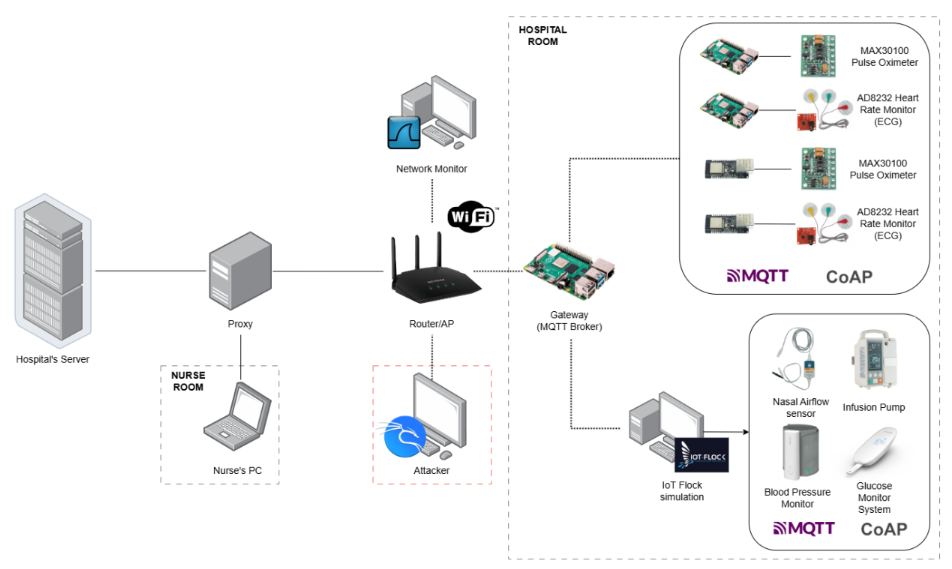
\includegraphics[width=1\textwidth]{img/MIOTTA_UPC.png}
    \caption{Esquema de l'arquitectura utilitzada. Imatge extreta del treball \cite{miottaupcfig}.}
    \label{fig:MQTT}
  \end{figure}

\section{Ús del protocol MQTT}
  Primer de tot, l’elecció del protocol MQTT (Message Queuing Telemetry Transport) està fonamentada en el fet que és un dels protocols més utilitzats en l’àmbit IoT en general i en entorns IoMT en específic.

  És un dels protocols amb més rellevància i eficiència per a dispositius amb recursos limitats, com és el cas d’aquest treball, on l’apartat de les comunicacions no és la seva funció principal. Consta d’una arquitectura \textit{publisher – subscriber} centralitzada en un únic servidor, la qual cosa fa que tota la informació estigui centralitzada en un sol dispositiu, aquest fet el fa vulnerable i, per tant, cal prendre les mesures de seguretat adequades. A més a més, és un protocol altament configurable, ja que s’hi poden configurar mesures de seguretat com ara limitacions de trànsit, Access Lists (ACL) o encriptat TLS.

  Dintre aquest projecte del grup ISG-UPC també es contempla el protocol CoAP, més enfocat a una arquitectura client -servidor semblant a protocols HTTP, però en aquest treball no serà utilitzat.

\section{Ús de Docker per al desplegament de dispositius}

  Per al desplegament dels dispositius simulats (clients) i del servidor MQTT (broker), s’ha optat per l’ús de contenidors Docker en lloc de màquines virtuals (VMs). Aquesta decisió s’ha pres tenint en compte diversos criteris tècnics, pràctics i de rendiment, que fan que Docker sigui una opció més adequada per als objectius del projecte.

  Docker et permet desplegar contenidors seguint una imatge comuna i configurable. D’aquesta manera, podem desplegar els clients simulats o el servidor en qualsevol entorn i sistema que compleixi uns requisits mínims de hardware I software. També permet mantenir una eficiència de recursos òptima, ja que utilitza el propi kernel del sistema hipervisor.

  Alhora, és un sistema aïllat del sistema operatiu principal, per això, podem executar proves de penetració sense veure compromesa realment la seguretat dels nostres equips i amb una gran facilitat de reproduir aquest atac diverses vegades sense haver de configurar novament tot el dispositiu vulnerat, ja que aquests contenidors són fàcilment renovables per còpies idèntiques prèvies a l'atac.
  
  A través del seu orquestrador Docker Compose, podem realitzar desplegaments múltiples de dispositius. Amb aquesta eina, podem desplegar en un sol dispositiu físic una gran quantitat de dispositius simulats que comparteixin unes característiques comunes entre ells.

  Dintre dels motius pels quals s’ha escollit aquesta tecnologia, està l’ús de volums, els quals et permeten compartir espai en memòria entre el dispositiu hipervisor i els contenidors. Aquesta funcionalitat ens permet agilitzar la transferència d’arxius entre contenidors, com ara fitxers de configuració, scripts per executar tasques determinades o atacs coordinats (en el cas de contenidors desplegats per l’atacant).

  També he utilitzat l’arquitectura de xarxa de Docker Compose per a poder crear infraestructures de xarxa simulades senceres, mantenint una lògica i rigorositat en les adreces de cada contenidor, d’aquesta manera, per a alguns atacs m’és possible simular una arquitectura com ara una gran quantitat de contenidors connectats a un switch o bé com un seguit de serveis del host per fer una arquitectura de microserveis dintre un mateix dispositiu.

  \begin{figure}[H]
    \centering
    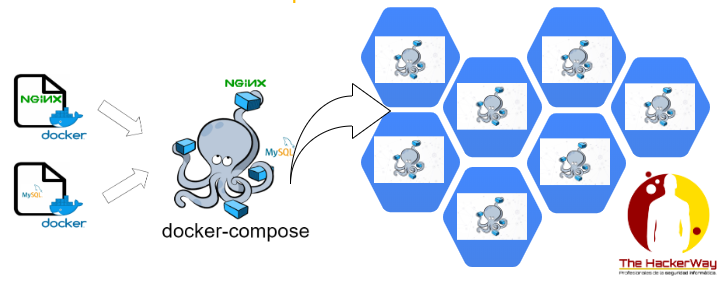
\includegraphics[width=1\textwidth]{img/DockerFig.png}
    \caption{Esquema de la generació de contenidors amb Docker Compose. Imatge extreta de \textit{The Hacker Way} \cite{miottaupcfig}.}
    \label{fig:MQTT2}
  \end{figure}

\section{Introducció d'expressions matemàtiques}
  
\LaTeX{} és una eina inestimable per a la composició tipogràfica de contingut matemàtic. En aquesta secció mostrem les comandes i entorns \LaTeX{} essencials per a l'escriptura matemàtica. Per a més informació consulteu el capítol 3 de "cita borrada".
  
\subsection{Matemàtiques en línia i aïllades}
  
Per a expressions en línia, utilitzeu \verb|$ ... $| o \verb|\( ... \)|. Escriviu entre \verb|\[ ... \]| les expressions que s'han de mostrar en una línia apart.


\ifcase\doclanguage\or
\begin{tcblisting}{colback=lime!10!white,colframe=gray!75!black,listing side text}
El polinomi $p(x) = 3x^2+2x-1$ t\'{e} arrels $x_1=-1$ i $x_2=\frac{1}{3}$.

Sigui la funci\'{o} de xarxa:
\[ H(s) = \frac{2\zeta\omega_o s}{s^2 + 2\zeta\omega_o s + \omega_o^2} \]
\end{tcblisting}%
%
\or
\begin{tcblisting}{colback=lime!10!white,colframe=gray!75!black,listing side text}
El polinomio $p(x) = 3x^2+2x-1$ tiene ra\'{i}ces $x_1=-1$ y $x_2=\frac{1}{3}$.

Sea la funci\'{o}n de red:
\[ H(s) = \frac{2\zeta\omega_o s}{s^2 + 2\zeta\omega_o s + \omega_o^2} \]
\end{tcblisting}
%
\else
\begin{tcblisting}{colback=lime!10!white,colframe=gray!75!black,listing side text}
The polynomial $p(x) = 3x^2 + 2x - 1$ has roots $x_1 = -1$ and $x_2 = \frac{1}{3}$.

Let the network function be:
\[ H(s) = \frac{2\zeta\omega_o s}{s^2 + 2\zeta\omega_o s + \omega_o^2} \]
\end{tcblisting}
\fi

\ifcase\doclanguage\or
  \subsection{Numeració i agrupació d'equacions}
  Els entorns \texttt{equation}, \texttt{gather}, \texttt{align} i altres numeren automàticament les equacions. Si definiu una etiqueta dins de l'equació podreu fer referència a ella dins del text usant \verb|\ref{etiqueta}|. Podeu suprimir la numeració amb \verb|\nonumber|.
\or
  \subsection{Numeración y agrupación de ecuaciones}
  Los entornos \texttt{equation}, \texttt{gather}, \texttt{align} y otros numeran automáticamente las ecuaciones. Si se define una etiqueta dentro de la ecuación se podrá hacer referencia a ella dentro del texto usando \verb|\ref{etiqueta}|. Se puede suprimir la numeración con \verb|\nonumber|.
\else
  \subsection{Equation Numbering and Grouping}
  The \texttt{equation}, \texttt{gather}, \texttt{align}, and other environments automatically number the equations. If you define a label within the equation, you can refer to it within the text using \verb|\ref{label}|. You can supress numbering with \verb|\nonumber|.
\fi

\begin{tcblisting}{colback=lime!10!white,colframe=gray!75!black,listing side text}
\begin{equation}
  a + b = c   \label{eq:formula}
\end{equation}
Xxxx xxx \ref{eq:formula}.

\begin{gather}
  c = a + b \\
  d + e = f   \nonumber
\end{gather}

\begin{align}
  c &= a + b \nonumber \\
  d + e &= f
\end{align}
\end{tcblisting}


\ifcase\doclanguage\or
  \subsection{Introducció de matrius}
\or
  \subsection{Introducción de matrices}
\else
  \subsection{Matrix Typesetting}
\fi
  
\begin{tcblisting}{colback=lime!10!white,colframe=gray!75!black,
  listing side text}
$A = \begin{pmatrix}
  a & b \\
  c & d
\end{pmatrix}$
\end{tcblisting}
  
\ifcase\doclanguage\or
  \section{Taules}
  
  El paquet \texttt{booktabs} (\cite{booktabs}) s'utilitza sovint per crear taules amb un espaiat millor i línies horitzontals més llegibles, i el paquet \texttt{array} es pot utilitzar per definir nous tipus de columna. A continuació es mostra un exemple de taula que utilitza aquests paquets i l'entorn \texttt{tabular} (consulteu el codi \LaTeX\ del document per a saber com s'ha creat.):
  
  \begin{table}[h]
    \centering
    \caption{Taula d'exemple}\label{tbl:taula1}
    \begin{tabular}{@{} l c >{\raggedright\arraybackslash}p{6.5cm} @{}}
      \toprule
      Element & Quantitat & Descripció \\
      \midrule
      Mango & 5 & Una fruita taronja \\
      Plàtan & 2 & Una fruita groga \\
      Cirera & 20 & Una fruita petita, rodona i vermella \\
      \bottomrule
    \end{tabular}
  \end{table}
  
  En aquest exemple (consulteu el codi font \LaTeX):
  
  \begin{itemize}
    \item \verb|\toprule|, \verb|\midrule|, i \verb|\bottomrule| del paquet \texttt{booktabs} creen línies horitzontals que tenen un espaiat per defecte millor que l'estàndard de \LaTeX\ \verb|\hline|.

    \item La definició \verb|>{\raggedright\arraybackslash}p{3cm}| del paquet \texttt{array} s'utilitza per crear un nou tipus de columna per a la descripció, on el text està alineat a l'esquerra i la columna té una amplada fixa de 3 cm.
  \end{itemize}
  
  Compileu aquest codi amb \LaTeX\ per produir la taula \ref{tbl:taula1}. La taula hauria de semblar bonica i llegible.

\or
\section{Tablas}
  
El paquete \texttt{booktabs} (\cite{booktabs}) se utiliza a menudo para crear tablas con un mejor espaciado y líneas horizontales más legibles, y el paquete \texttt{array} se puede usar para definir nuevos tipos de columnas. Aquí hay un ejemplo de tabla utilizando estos paquetes y el entorno \texttt{tabular} (consultar el código fuente del documento para ver cómo se ha creado):
  
\begin{table}[h]
  \centering
  \caption{Tabla de Ejemplo}\label{tbl:tabla1}
  \begin{tabular}{@{} l c >{\raggedright\arraybackslash}p{6cm} @{}}
    \toprule
    Artículo & Cantidad & Descripción \\
    \midrule
    Manzana & 5 & Una fruta roja \\
    Plátano & 2 & Una fruta amarilla \\
    Cereza & 20 & Una fruta pequeña, redonda y roja \\
    \bottomrule
  \end{tabular}
\end{table}
  
En este ejemplo (consultar el código fuente \LaTeX):
  
\begin{itemize}
  \item \verb|\toprule|, \verb|\midrule| y \verb|\bottomrule| del paquete \texttt{booktabs} crean líneas horizontales que tienen un mejor espaciado por defecto que el estándar de LaTeX \verb|\hline|.
  
  \item La definición \verb|>{\raggedright\arraybackslash}p{3cm}| del paquete \texttt{array} se usa para crear un nuevo tipo de columna para la descripción, donde el texto está alineado a la izquierda y la columna tiene un ancho fijo de 3 cm.
\end{itemize}
  
Compilar este código con \LaTeX\ para producir la tabla \ref{tbl:tabla1}. La tabla debería lucir hermosa y legible.

\else
  \section{Tables}
  
  The \texttt{booktabs} package (\cite{booktabs}) is often used to create tables with better spacing and more readable horizontal lines, and the \texttt{array} package can be used to define new column types. Here's an example table using these packages and the \texttt{tabular} environment (look at the \LaTeX\ code to see how it's created):
  
  \begin{table}[h]
    \centering
    \caption{Example Table}\label{tbl:table1}
    \begin{tabular}{@{} l c >{\raggedright\arraybackslash}p{5cm} @{}}
      \toprule
      Item & Quantity & Description \\
      \midrule
      Apple & 5 & A red fruit \\
      Banana & 2 & A yellow fruit \\
      Cherry & 20 & A small, round, red fruit \\
      \bottomrule
    \end{tabular}
  \end{table}
  
  In this example (see the \LaTeX\ source code):
  
  \begin{itemize}
    \item \verb|\toprule|, \verb|\midrule|, and \verb|\bottomrule| from the \texttt{booktabs} package create horizontal lines that have better default spacing than LaTeX's standard \verb|\hline|.

    \item The \texttt{array} package's \verb|>{\raggedright\arraybackslash}p{3cm}| definition is used to create a new column type for the description, where the text is left-aligned and the column has a fixed width of 3 cm.
  \end{itemize}
  
  Compile this code with \LaTeX\ to produce the table \ref{tbl:table1}. The table should look beautiful and readable.
\fi

\ifcase\doclanguage\or
  \section{Diagrames}
    El paquet \textit{TikZ} (\cite{tikz}) permet dibuixar tot tipus de diagrames i gràfics. Val la pena consultar el seu manual d'ús per tal de conèixer el seu funcionament i poder-ne treure tot el suc possible. Cal no deixar-se intimidar per la seva longitud (1300+ pàgines) ja que la majoria d'espai l'ocupen nombrosos exemples que il·lustren les possibilitats del llenguatge.
    
    Per si això fos poc, també hi ha disponibles una sèrie de biblioteques addicionals que permeten d'augmentar encara més les funcionalitats del \textit{TikZ} amb l'addició d'ordres per facilitar el dibuix de tot tipus d'objectes, des de xarxes de Petri fins a circuits electrònics, passant per coses tan diverses com calendaris, diagrames d'estats o figures de papiroflèxia.
    
    La figura \ref{fig:tikz} mostra alguns exemples de diagrames creats amb el paquet \textit{TikZ}.

\or
\section{Diagramas}
  El paquete \textit{TikZ} (\cite{tikz}) permite dibujar todo tipo de diagramas y gráficos. Vale la pena consultar su manual de usuario para entender cómo funciona y aprovechar al máximo sus posibilidades. No cabe dejarse intimidar por su longitud (más de 1300 páginas) ya que la mayoría del espacio está ocupado por numerosos ejemplos que ilustran las capacidades del lenguaje.
  
  Por si eso fuera poco, también hay varias bibliotecas adicionales disponibles que mejoran aún más la funcionalidad de \textit{TikZ} con comandos adicionales para dibujar diversos objetos, desde redes de Petri hasta circuitos electrónicos, cubriendo temas diversos como calendarios, diagramas de estados o figuras de origami.
  
  La figura \ref{fig:tikz} muestra algunos ejemplos de diagramas creados con el paquete \textit{TikZ}.

\else
\section{Diagrams}
  The package \textit{TikZ} (\cite{tikz}) allows you to draw all kinds of diagrams and graphics. It's worth consulting its user manual to understand how it works and make the most of it. Don't be intimidated by its length (1300+ pages) because most of the space is filled with numerous examples illustrating the language's capabilities.
  
  As if that were not enough, there are also several additional libraries available that further enhance \textit{TikZ}'s functionality with additional commands for drawing various objects, from Petri nets to electronic circuits, covering diverse topics such as calendars, state diagrams, or origami figures.
  
  The figure \ref{fig:tikz} shows some examples of diagrams created using the \textit{TikZ} package.

\fi

\begin{figure}[ht]
  \centering
  \begin{tikzpicture}[scale=1,angle radius=.75cm]
    \node (A) at (-2,0)     [red,left]   {$A$};
    \node (B) at ( 3,.5)    [red,right]  {$B$};
    \node (C) at (-2,2)     [blue,left]  {$C$};
    \node (D) at ( 3,2.5)   [blue,right] {$D$};
    \node (E) at (60:-5mm)  [below]      {$E$};
    \node (F) at (60:3.5cm) [above]      {$F$};
    \coordinate (X) at (intersection cs:first line={(A)--(B)}, second line={(E)--(F)});
    \coordinate (Y) at (intersection cs:first line={(C)--(D)}, second line={(E)--(F)});
    \path
    (A) edge [red, thick]  (B)
    (C) edge [blue, thick] (D)
    (E) edge [thick]       (F)
    pic ["$\alpha$", draw, fill=yellow]   {angle = F--X--A}
    pic ["$\beta$", draw, fill=green!30] {angle = B--X--F}
    pic ["$\gamma$", draw, fill=yellow]   {angle = E--Y--D}
    pic ["$\delta$", draw, fill=green!30] {angle = C--Y--E};
    \node at ($ (D)!.5!(B) $) [right=1cm,text width=6cm,rounded corners,fill=red!20,inner sep=1ex]
    {
      When we assume that $\color{red}AB$ and $\color{blue}CD$ are
      parallel, i.\,e., ${\color{red}AB} \mathbin{\|} \color{blue}CD$,
      then $\alpha = \gamma$ and $\beta = \delta$.
    };
  \end{tikzpicture}\\
  \begin{tikzpicture}
    \tikzset{
      molla/.style    = {thick,decorate,decoration={coil,aspect=0.9,pre length=0.3cm,post length=0.3cm,segment length=5}},
      terra/.style    = {fill,pattern=north east lines,draw=none,minimum width=0.75cm,minimum height=0.3cm},
      amortidor/.style= {thick,decoration={markings,  
          mark connection node=dmp,
          mark=at position 0.5 with 
          {
            \node (dmp) [thick,inner sep=0pt,transform shape,rotate=-90,minimum width=15pt,minimum height=3pt,draw=none] {};
            \draw [thick] ($(dmp.north east)+(2pt,0)$) -- (dmp.south east) -- (dmp.south west) -- ($(dmp.north west)+(2pt,0)$);
            \draw [thick] ($(dmp.north)+(0,-5pt)$) -- ($(dmp.north)+(0,5pt)$);
          }
        }, decorate
      },
    }
    \node[draw,outer sep=0pt,thick] (M) [minimum width=1cm, minimum height=2cm] {$M$};
    \node (ground) [terra,anchor=north,yshift=-0.25cm,minimum width=1.5cm] at (M.south) {};
    \draw (ground.north east) -- (ground.north west);
    \draw [thick] (M.south west) ++ (0.2cm,-0.125cm) circle (0.125cm)  (M.south east) ++ (-0.2cm,-0.125cm) circle (0.125cm);
    
    \node (wall) [terra, rotate=-90, minimum width=3cm,yshift=-3cm] {};
    \draw (wall.north east) -- (wall.north west);
    
    \draw [molla] (wall.165) -- node[pos=0.5,above] {$K$} ($(M.north west)!(wall.165)!(M.south west)$);
    \draw [amortidor] (wall.15) -- node[pos=0.5,yshift=0.5cm] {$B$} ($(M.north west)!(wall.15)!(M.south west)$);
    
    \draw [-latex,ultra thick] (M.east) ++ (0.2cm,0) -- +(1cm,0) node[anchor=west]{$f(t)=k_m\cdot i(t)$};
    
    \draw [-latex,ultra thick] (M.north east) ++ (0,0.1cm) 
    -- ++(0,0.5cm) -- ++(0.5cm,0) node[anchor=west] {$x(t)$};
  \end{tikzpicture}\\
  \begin{circuitikz}[american, decoration={coil}]
    \draw (0,0) circle[radius=1cm] circle[radius=1.5cm];
    \draw [->,thick](0,0) -- node[midway, left]{R}(80:1.5) ;
    \draw [->,thick](0,0) --node[midway,below]{r}(30:1); 
    \begin{scope}
      \draw[decorate, decoration={aspect=0.4, segment length=3mm, amplitude=5mm}]
      (1.25,-0.8) coordinate (a) --node[midway,right=0.5cm]{$V_2$} + (0,2) coordinate (b);
      \draw[decorate, decoration={aspect=0.4, segment length=5mm, amplitude=5mm}]
      (-1.25,-0.8) coordinate (c) --node[midway,left=0.5cm]{$V_1$} + (0,2) coordinate (d);
    \end{scope}
    % left circuit
    \draw (-5,1.0) coordinate (e2) to[battery2,v=$V_{cc}$] (-5,-1.0) coordinate(e1);
    \draw (e1) to[R,l=$R_1$,-] (e1-|c) --(c)node[below=0.5cm]{$N_1$};
    \draw(e2)-- (d-|e2) to[short,i>=$I$] (d);
    % right circuit
    \draw (5,1) coordinate(e3) to[C=C,v=$V$,-*] (5,-1) coordinate (e4);
    \draw  (b) to[R=$R_2$,i=$i$,-*] (b-|e3)--(e3);
    \draw   (e4) to[short] (a|-e4)--(a) node[below=0.5cm]{$N_2$};
    
  \end{circuitikz}
   \caption{%
     \ifcase\doclanguage\or%
       Diagrames creats usant les ordres del paquet \emph{TikZ}
     \or
       Diagramas creados usando les ordres del paquet \emph{TikZ}
     \else
       Diagrams created using the commands provided by the \emph{TikZ} package
     \fi%
   }\label{fig:tikz}
\end{figure}

\ifcase\doclanguage\or
  \section{Gràfiques}
  
  Òbviament podeu crear les vostres gràfiques usant un programa informàtic adient, exportant el resultat a algun format gràfic (preferiblement vectorial com ara PDF per no perdre qualitat) i inserint les imatges resultants al document \LaTeX\ en la forma habitual. Aquesta via, però, té l'inconvenient que dificulta aconseguir la coherència i cohesió tipogràfica entre el text del document i el de les imatges. Com a conseqüència, la qualitat del document se'n ressent.
  
  Per tant, si es vol aconseguir la màxima coherència tipogràfica entre el text i les gràfiques, és preferible que sigui el propi \LaTeX\ qui s'encarregui de generar les gràfiques (amb les dades que li proporcionem) ja que en aquest cas usarà les mateixes fonts arreu del document.
  
  A tal efecte al llarg dels anys s'han desenvolupat múltiples paquets i tècniques per aconseguir aquest objectiu. El que aquí us proposem és usar el paquet «\textbf{pgfplots}», que utilitza internament el paquet \textit{TikZ} per generar una sèrie de \textit{macros} addicional que faciliten el dibuix de gràfiques. La figura \ref{fig:plot} mostra un exemple del que es pot arribar a fer amb aquest paquet, però recomanem fermament que consulteu el manual d'instruccions (\cite{pgfplots}) on s'il·lustren molts més exemples.
\or
  \section{Gráficas}
  
  Obviamente, pueden crear sus gráficos utilizando un programa informático adecuado, exportando el resultado a algún formato gráfico (preferiblemente vectorial, como PDF, para no perder calidad) e insertando las imágenes resultantes en el documento \LaTeX\ de la forma habitual. Sin embargo, esta opción tiene la desventaja de dificultar la coherencia y cohesión tipográfica entre el texto del documento y el de las imágenes. Como consecuencia, la calidad del documento se ve afectada.
  
  Por lo tanto, si se busca lograr la máxima coherencia tipográfica entre el texto y los gráficos, es preferible que sea el propio \LaTeX\ el que se encargue de generar los gráficos (con los datos que le proporcionemos), ya que en este caso utilizará las mismas fuentes en todo el documento.
  
  Con este fin, a lo largo de los años se han desarrollado múltiples paquetes y técnicas para lograr este objetivo. Lo que aquí les proponemos es utilizar el paquete «\textbf{pgfplots}», que utiliza internamente el paquete \textit{TikZ} para generar una serie de \textit{macros} adicionales que facilitan el dibujo de gráficos. La figura \ref{fig:plot} muestra un ejemplo de lo que se puede llegar a hacer con este paquete, pero recomendamos encarecidamente que consulten el manual de instrucciones (\cite{pgfplots}), donde se ilustran muchos más ejemplos.
\else
  \section{Plotting}
  
  Obviously, you can create your graphs using suitable software, exporting the result to a graphic format (preferably vectorial, such as PDF, to avoid loss of quality) and then inserting the resulting images into the \LaTeX\ document in the usual way. However, this approach has the disadvantage of making it difficult to achieve typographic coherence and cohesion between the document text and the images. As a result, the document's quality may suffer.
  
  Therefore, if you aim to achieve maximum typographic coherence between the text and the graphics, it is preferable to let \LaTeX\ itself generate the graphics (using the data you provide), as it will use the same fonts throughout the document.
  
  To this end, over the years, various packages and techniques have been developed to achieve this goal. What we propose here is to use the \textbf{pgfplots} package, which internally uses the \textit{TikZ} package to generate a set of additional macros that facilitate the drawing of graphs. Figure \ref{fig:plot} shows an example of what can be done with this package, but we strongly recommend consulting the instruction manual (\cite{pgfplots}), which illustrates many more examples.
\fi

\begin{figure}[ht]
  \centering
  \begin{tikzpicture}
  \tikzset{
    every pin/.style={fill=yellow!20!white,rectangle,rounded corners=3pt,inner sep=3pt,font=\scriptsize},
    small dot/.style={fill=black,circle,scale=0.25},
  }
  \begin{semilogxaxis}[
    width=14cm,
    height=10cm,
    grid=both,
    xmin=1,
    xmax=1E8,
    ymin=5,
    ymax=55,
    xlabel={\ifcase\doclanguage\or Freqüència\or Frecuencia\else Frequency\fi [\si{\Hz}]},
    ylabel={\ifcase\doclanguage\or Guany\or Ganancia\else Gain\fi [\si{\dB}]},
    every tick label/.append style={font=\scriptsize},
    extra y ticks={41.7},
    extra y tick labels={\SI{41,7}{\dB}},
    extra y tick style={color=red,grid style={color=red}},
  ]
    \addplot[color=blue,line width=1pt] table[x index=0, y index=1,search path={data}] {RF-lineal.dat}
      node[pin={[pin distance=0.5cm]135:{$G_{max}=\SI{44,64}{\dB}$}},fill,circle,scale=0.5] at (axis cs:1000,44.64) {}
    ;
    \addplot[color=red,line width=1pt] table[x index=0, y index=1,search path={data}] {RF-model-SPICE-adaptat.dat}
      node[pin={[pin distance=0.5cm]-70:{$G_{max}=\SI{44,76}{\dB}$}},fill,circle,scale=0.5] at (axis cs:2000,44.76) {}
    ;
    \node[pin={[pin distance=1cm]-45:{$f_{c1}\simeq\SI{15}{\Hz}$}},fill,circle,scale=0.5] at (axis cs:15.2,41.7) {};
    \addlegendentry{\ifcase\doclanguage\or
      Model lineal en petit senyal\or
      Modelo lineal en pequeña señal\else
      Small-signal linear model\fi
    };
    \addlegendentry{\ifcase\doclanguage\or
      Macromodel SPICE\or
      Macromodelo SPICE\else
      SPICE Macromodel\fi
    };
    \fill[white] (1.4cm,1cm) rectangle (9.4cm,5.5cm);
  \end{semilogxaxis}
  \begin{semilogxaxis}[
    name=detall,
    width=8cm,
    height=5cm,
    at={(2.5cm,0.5cm)},
    anchor=south west,
    axis background/.style={fill=black!05!white},
    title={\ifcase\doclanguage\or 
      Detall al voltant de\or
      Detalle alrededor de\else
      Detail around\fi\ 
      \SI{500}{\kHz}
    },
    title style={yshift=-5pt},
    grid=both,
    % Eix X
    xmin=1E5,
    xmax=1E6,
    xtick={1e5,2e5,3e5,4e5,5e5,6e5,7e5,8e5,9e5,1e6},
%     xtick={1e5,5e5,1e6},
    xticklabels={\SI{100}{\kHz},,,,\SI{500}{\kHz},,,,,\SI{1}{\MHz}},
    every axis x label/.style={at={(ticklabel* cs:1.06)},anchor=north west,},
%     xlabel=(Hz),
    % Eix Y
    ymin=38,
    ymax=46,
    every tick label/.append style={font=\scriptsize},
    ytick={38,40,44},
    yticklabels={\SI{38}{\dB},\SI{40}{\dB},\SI{44}{\dB}},
    extra y ticks={41.7,44.7},
    extra y tick labels={\SI{41,7}{\dB},\SI{44,7}{\dB}},
    extra y tick style={color=red,grid style={color=red}},
%     ylabel=(dB),
  ]
    \addplot[color=blue,line width=1.5pt] table[x index=0, y index=1,search path={data}] {RF-lineal.dat}
    node[pin={[pin distance=0.5cm]-155:{$f_{c2}\simeq\SI{556}{\kHz}$, $G\simeq\SI{41.64}{\dB}$}},fill,circle,scale=0.5] at (axis cs:556e3,41.64) {};
    \addplot[color=red,line width=1.5pt] table[x index=0, y index=1,search path={data}] {RF-model-SPICE-adaptat.dat}
    node[pin={[pin distance=0.8cm]-100:{$f_{c2}\simeq\SI{708}{\kHz}$, $G\simeq\SI{41.76}{\dB}$}},fill,circle,scale=0.5] at (axis cs:708e3,41.76) {};
  \end{semilogxaxis}
\end{tikzpicture}

  \caption{\ifcase\doclanguage\or
     Exemple de gràfica complexa dibuixada amb ajut del paquet \emph{pgfplots}\or
     Ejemplo de un gráfico complejo dibujado con la ayuda del paquete \emph{pgfplots}\else
     Example of a complex graph drawn using the \emph{pgfplots} package\fi
  }\label{fig:plot}
\end{figure}

\ifcase\doclanguage\or
  \section{Llistats de codi}
  
  L'entorn \texttt{tcblistings} del paquet \texttt{tcolorbox} (\cite{tcolorbox}) insereix els llistats de codi generats pels paquets \texttt{listings} o \texttt{minted} dins d'una \texttt{tcolorbox}, amb la qual cosa s'aconsegueixen uns llistats molt ben presentats i altament configurables.
  
  Com a exemple d'això, a continuació es mostra el llistat d'un programa en llenguatge Python que implementa l'algorisme del «sedàs d'Eratòstenes» per calcular els nombres primers menors d'un cert nombre donat. Observeu que el paquest «listings» és capaç d'interpretar i ressaltar automàticament la sintaxi del llenguatge.
\or
  \section{Listados de código}

  El entorno \texttt{tcblistings} del paquete \texttt{tcolorbox} (\cite{tcolorbox}) inserta los listados de código generados por los paquetes \texttt{listings} o \texttt{minted} dentro de una \texttt{tcolorbox}, con lo cual se consiguen unos listados muy bien presentados y altamente configurables.

  Como ejemplo de esto, a continuación se muestra el listado de un programa en lenguaje Python que implementa el algoritmo de la «criba de Eratóstenes» para calcular los números primos menores de cierto número dado. Observar que el paquete «listings» es capaz de interpretar y resaltar automáticamente la sintaxis del lenguaje.
\else
  \section{Code Listings}

  The \texttt{tcblistings} environment of the \texttt{tcolorbox} package (\cite{tcolorbox}) inserts code listings generated by the \texttt{listings} or \texttt{minted} packages into a \texttt{tcolorbox}, thereby achieving very well-presented and highly con\-fi\-gu\-ra\-ble listings.

  As an example, the following is the listing of a program in Python language that implements the "Sieve of Eratosthenes" algorithm for calculating prime numbers less than a certain given number. Note that the "listings" package is capable of automatically interpreting and highlighting the language's syntax.
\fi

\newcommand\ListTitle{\ifcase\doclanguage\or
  Exemple de Python: Sedàs d'Eratòstenes\or
  Ejemplo de Python: Criba de Eratóstenes\else
  Python Example: Sieve of Eratosthenes\fi
}
\begin{tcblisting}{colback=gray!5!white,colframe=gray!75!black,listing only,
    title=\ListTitle, fonttitle=\bfseries, breakable, enhanced jigsaw, leftupper=8mm,
    listing options={language=python,basicstyle=\ttfamily\small,
    showstringspaces=false, numbers=left, numberstyle=\footnotesize, stepnumber=1, numbersep=8pt}}
def sieve_of_eratosthenes(limit):
  primes = []
  sieve = [True] * (limit + 1)
  for num in range(2, limit + 1):
    if sieve[num]:
      primes.append(num)
      for multiple in range(num*num, limit + 1, num):
        sieve[multiple] = False
  return primes

# Example usage:
if __name__ == "__main__":
  limit = 30
  print(f"The prime numbers up to {limit} are:
          {sieve_of_eratosthenes(limit)}")
\end{tcblisting}

\ifcase\doclanguage\or
  \section{Unitats}
  
  Una de les coses que sovint es menysté a l'hora d'escriure és la correcta representació de valors i unitats, que és essencial en textos científics i tècnics. El paquet \texttt{siunitx} de \LaTeX\ s'ajusta al sistema internacional d'unitats (SI) i amb ell els usuaris poden assegurar-se que els nombres i unitats són presentats amb la notació, espaiat i font adequats, tot respectant les diferents convencions internacionals.
  
  A continuació presentem alguns exemples d'ús, però per una presentació exhaustiva de les possibilitats del paquet caldrà que consulteu la seva documentació (\cite{siunitx}).
  
  \begin{itemize}
    \item \textbf{Composició tipogràfica d'unitats senzilles}: Per composar una unitat utilitzant \texttt{siunitx}, podeu fer servir la comanda \verb|\si{}|. Per exemple, per composar "metres per segon," escriuríeu:
       \verb|\si{\meter\per\second}| que resultaria en «\si{\meter\per\second}» amb l'espaiament correcte entre ells.
    
    \item \textbf{Combinació de Nombre i Unitat}: Si voleu incloure un valor amb una unitat, useu la comanda \verb|\SI{}|. Per exemple, per expressar "10 kilo-ohm" escriuríeu:
       \verb|\SI{10}{\kohm}|, que resulta en \SI{10}{\kohm}. Aquesta comanda assegura que el nombre i la unitat estan adequadament espaiats.
    
    \item \textbf{Unitats complexes}: Per unitats més complexes, \texttt{siunitx} permet combinar unitats de diverses maneres. Per exemple, per composar «gigawatts per metre quadrat per estereoradian» podeu usar:
    
    \verb|\si{\giga\watt\per\square\meter\per\steradian}|
    
    i el paquet treu «\si{\giga\watt\per\square\meter\per\steradian}» tenint cura de tota la formatació adequada i la font.
  \end{itemize}

  \texttt{siunitx} és molt flexible i pot manejar una àmplia gamma d'unitats i opcions de formatatge de nombres, incloent nombres complexos amb unitats, l'alineació en taules, l'arrodoniment de nombres, i l'establiment d'opcions globals per a la consistència a través d'un document.
\or
  \section{Unidades}
  
  Una de las cosas que a menudo se pasa por alto al escribir es la correcta representación de valores y unidades, lo cual es esencial en textos científicos y técnicos. El paquete \texttt{siunitx} de \LaTeX\ se ajusta al sistema internacional de unidades (SI) y con él, los usuarios pueden asegurarse de que los números y unidades se presenten con la notación, espaciado y fuente adecuados, respetando las diferentes convenciones internacionales.
  
  A continuación, presentamos algunos ejemplos de uso, pero para una presentación exhaustiva de las posibilidades del paquete, deberás consultar su documentación (\cite{siunitx}).
  
  \begin{itemize}
      \item \textbf{Composición tipográfica de unidades simples}: Para componer una unidad utilizando \texttt{siunitx}, puedes usar el comando \verb|\si{}|. Por ejemplo, para componer «metros por segundo», escribirías: \verb|\si{\meter\per\second}|, lo que resultaría en «\si{\meter\per\second}» con el espaciado correcto entre ellos.
  
      \item \textbf{Combinación de Número y Unidad}: Si se quiere incluir un valor con una unidad, utiliza el comando \verb|\SI{}|. Por ejemplo, para expresar «10 kilo-ohmios», se escribiría: \verb|\SI{10}{\kohm}|, lo que resulta en \SI{10}{\kohm}. Este comando asegura que el número y la unidad estén adecuadamente espaciados.
  
      \item \textbf{Unidades complejas}: Para unidades más complejas, \texttt{siunitx} permite combinar unidades de diversas maneras. Por ejemplo, para componer «gigavatios por metro cuadrado por estereorradian», puedes usar:
      
      \verb|\si{\giga\watt\per\square\meter\per\steradian}|
      
      y el paquete genera «\si{\giga\watt\per\square\meter\per\steradian}» cuidando de toda la formatación adecuada y la fuente.
  
  \end{itemize}
  
  \texttt{siunitx} es muy flexible y puede manejar una amplia gama de unidades y opciones de formateo de números, incluso complejos, incluyendo la alineación en tablas, el redondeo de números y el establecimiento de opciones globales para la consistencia a lo largo de un documento.
  
\else
  \section{Units}
  
  One of the things that is often overlooked when writing is the correct representation of values and units, which is essential in scientific and technical texts. The \texttt{siunitx} package in \LaTeX\ conforms to the International System of Units (SI), and with it, users can ensure that numbers and units are presented with the appropriate notation, spacing, and font, while respecting different international conventions.

  Below, we present some usage examples, but for a comprehensive overview of the package's capabilities, you should refer to its documentation (\cite{siunitx}).

  \begin{itemize}
    \item \textbf{Typesetting Simple Units}: To typeset a unit using \texttt{siunitx}, you can use the command \verb|\si{}|. For example, to compose "meters per second," you would write: \verb|\si{\meter\per\second}|, resulting in «\si{\meter\per\second}» with the correct spacing between them.

    \item \textbf{Combining Numbers and Units}: If you want to include a value with a unit, use the \verb|\SI{}| command. For instance, to write "10 kilo ohm" you would write: \verb|\SI{10}{\kohm}|, resulting in \SI{10}{\kohm}. This command ensures that the number and unit are appropriately spaced.

    \item \textbf{Complex Units}: For more complex units, \texttt{siunitx} allows you to combine units in various ways. For example, to compose "gigawatts per square meter per steradian", you can use: 
    
    \verb|\si{\giga\watt\per\square\meter\per\steradian}|
    
    and the package produces «\si{\giga\watt\per\square\meter\per\steradian}» while taking care of all the proper formatting and font.
  \end{itemize}

  \texttt{siunitx} is highly flexible and can handle a wide range of units and number formatting options, including complex numbers with units, alignment in tables, rounding of numbers, and setting global options for consistency throughout a document.
\fi